\documentclass[]{article}
\usepackage{amsmath}
\usepackage{amsfonts}
\usepackage{amssymb}
\usepackage{algorithmic}
\usepackage{algorithm}
\usepackage{tikz}
\usepackage{graphicx}
\usepackage{mdframed}
\usepackage{paralist}
\usepackage{listings}

\definecolor{dkgreen}{rgb}{0,0.6,0}
\definecolor{gray}{rgb}{0.5,0.5,0.5}

\lstset{
  language=Python,
  breaklines=true,
  showstringspaces=false,
  frame=single,
  aboveskip=3mm,
  belowskip=3mm,
  columns=flexible,
  basicstyle={\small\ttfamily},
  numbers=none,
  numberstyle=\tiny\color{gray},
  keywordstyle=\color{blue},
  commentstyle=\color{gray},
  stringstyle=\color{dkgreen},
  breakatwhitespace=true,
  tabsize=3
}

\title{CAGD - Homework 3}
\author{Josefine St{\aa}l \& Erik Ackzell}

\begin{document}

\maketitle

\section*{Task 1}
As we understood the task we want to give all the basis functions for the two knot sequences $U_1=\{0,0,1,1\}$ and $U_2=\{0,0,0,1,1,1\}$. We use the recursion formula for calculating the basis functions for each index $i$,
$$N_i^0(u)=\left\{ \begin{array}{ll}
1, & \text{if } u\in [u_i,u_{i+1}) \\
0, & \text{else} \end{array}\right.$$
$$N_i^n(u)=\frac{u-u_i}{u_i+n-u_i}N_i^{n-1}+\frac{u_{i+n+1}-u}{u_{i+n+1}-u_{i+1}}N_{i+1}^{n+1}(u)$$
where $u_i$ are the knots. We can easily calculate how many basis functions there are for each degree by the relation $$\#\text{knots}-1=\text{degree}+\#\text{basis functions}$$ 
The basis functions for $U1=\{0,0,1,1\}$ are the following:
$$N_0^1(u)=(1-u)N_1^0(u)$$
$$N_1^1(u)=uN_1^0(u)$$
$$N_0^2(u)=2u(1-u)N_1^0(u)$$
The basis functions for $U2=\{0,0,0,1,1,1\}$ are as follows:
$$N_0^1(u)=0$$
$$N_1^1(u)=(1-u)N_2^0(u)$$
$$N_2^1(u)=uN_2^0(u)$$
$$N_3^1(u)=0$$
$$N_0^2(u)=(1-u)^2N_2^0(u)$$
$$N_1^2(u)=2u(1-u)N_2^0(u)$$
$$N_2^2(u)=u^2N_2^0(u)$$
$$N_0^3(u)=3u(1-u)^2N_2^0(u)$$
$$N_1^3(u)=3u^2(1-u)N_2^0(u)$$
$$N_0^4(u)=6u^2(1-u)^2N_2^0(u)$$
As can be seen by the basis functions above we have a clear pattern in the coefficents to and the multiples of $u$ and $(1-u)$ respectively.

\section*{Task 2}
The algorithm that calculates and plots the values of the basis functions corresponding to any given knot sequence and degree, can be found in Appendix I. In this task the degree is $2$ and the knot sequence $\{0,0,0,0.3,0.5,0.5,0.6,1,1,1\}$.
\begin{figure}[h!]
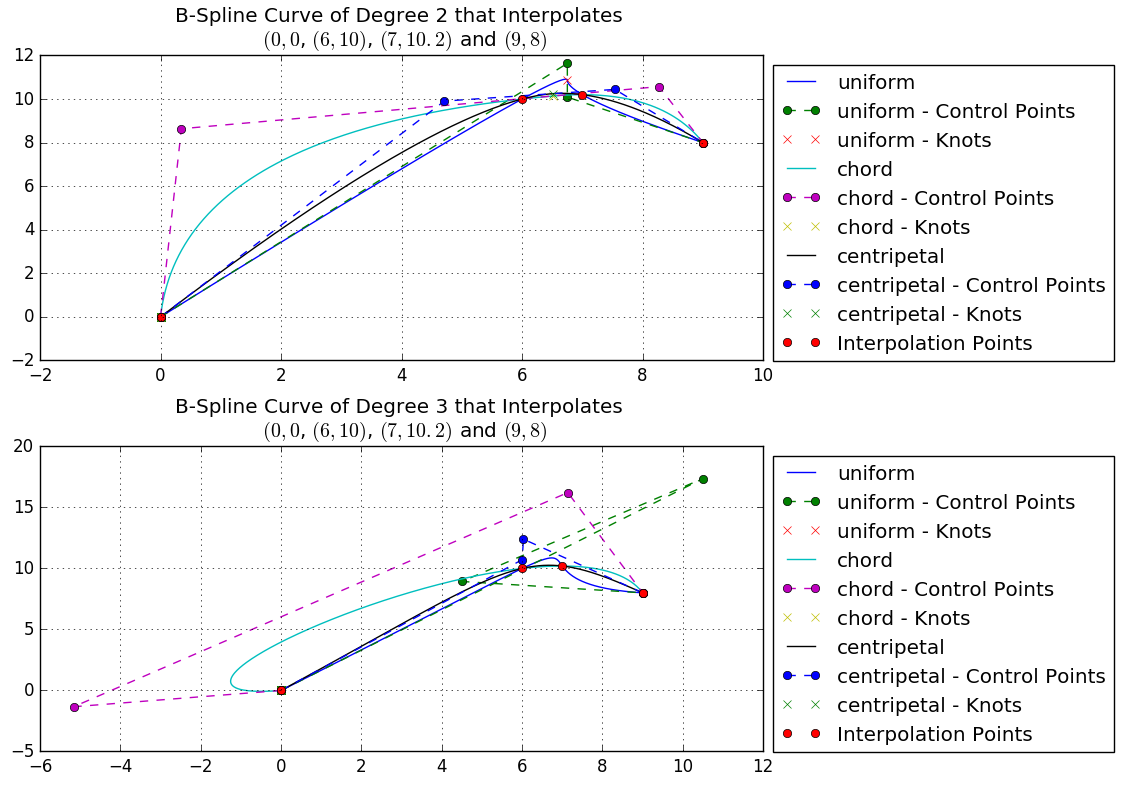
\includegraphics[scale=0.6]{task2}
\end{figure}


\section*{Task 3}
In this task we implement a method to check whether a real number is in an interval with full support, given a knot sequence, a degree of the spline basis and the number itself. The code can be seen in Appendix 1. \\
We tried our code for three different knot sequences, $k_1=(0, 0, 1, 1)$, $k_2=(0, 0, 0, 1, 1, 1)$ and $k_3=(0, 0, 0, 0.3, 0.5, 0.6, 1, 1, 1)$, all with quadratic splines. For each of the scenarios, we tested our code with the real numbers $\{0.12, 0.24, 0.4, 0.53, 0.78, 0.8\}$.
\begin{itemize}
	\item For $k_1$, we found that all points were in intervals \textbf{without} full support.
	\item For $k_2$, we found that all points were in intervals \textbf{with} full support.
	\item For $k_3$, we found that all points were in intervals \textbf{with} full support.
\end{itemize}
The results were as expected, as an interval has full support when using quadratic splines, if there are 3 or more knots to the left of the interval as well as to the right of the interval.

%\begin{figure}[h!]
%	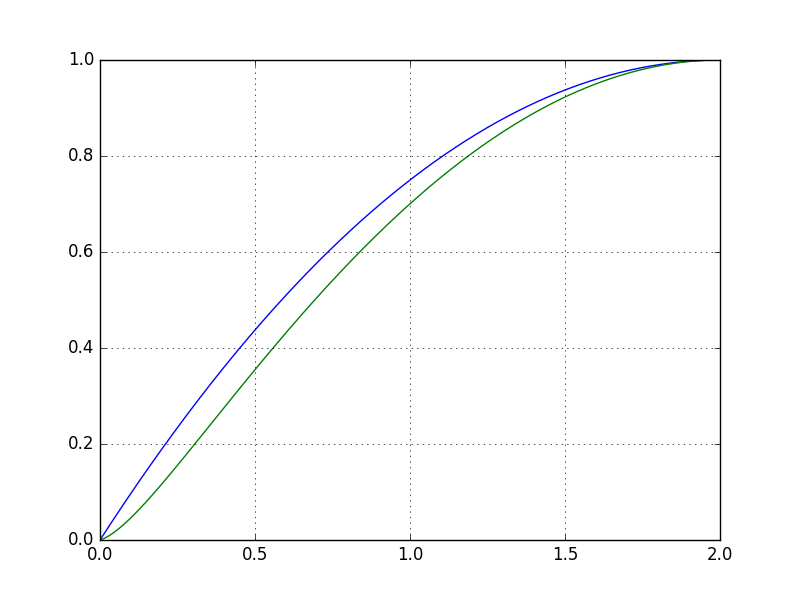
\includegraphics[scale=0.6]{non_symmetric_degree_elevation}
%\end{figure}


\newpage
\section*{Appendix I}
%\lstinputlisting[lastline=347]{beziercurveclass.py}

\end{document}
